\documentclass[a4paper,11pt,dvipdfmx]{ujarticle}
% パッケージ
\usepackage{graphicx}
\usepackage{url}
% レイアウト指定を記述したファイルの読み込み
\input{layout}

% タイトルと氏名を変更せよ.
\title{日本におけるデジタル化の状況}
\author{G584852025 丸山 惟央}

\begin{document}

\maketitle %

% ここから本文
\section{デジタル競争力ランキング}
% を使う
国際経営開発研究所(IMD)の調査\cite{oecd}によると,日本のデジタル競争力のランキングは図\ref{fig:加入率}に示すように,調査対象の64カ国中,総合で28位,準備分野で27位となっている.

\begin{figure}[htbp]
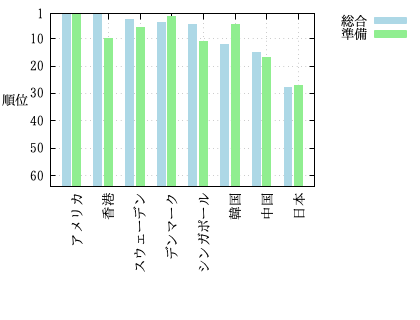
\includegraphics{G584852025.png}
\centering
\caption{デジタル競争力ランキング(64カ国中)}\label{fig:加入率}
\end{figure}














\section{ブロードバンドの整備状況}
OECDによるブロードバンド回線の普及に関する調査\cite{imd}によると,表\ref{tbl:利用状況}に示すように,日本における100人あたりのモバイルブロードバンドの加入者数は 190.5で,第1位になっている.2位はエストニアで,3位米国へと続く.




\begin{table}[htbp]
    \centering
    \caption{インターネット端末の利用状況}
    \label{tbl:利用状況}

    \begin{tabular}{|c|l|r|}\hline
        順位 & 国名 & 加入者数\\
        \hline
        1位 & 日本   & 190.5 \\
        \hline
        2位 & エストニア  & 179.9 \\
        \hline
        3位 & 米国  & 169.0 \\
        \hline
        4位 & フィンランド  & 157.0 \\
        \hline
        5位 & デンマーク  & 141.7 \\
        \hline
        6位 & ラトビア  & 141.6 \\
        \hline 
        7位 & イスラエル  & 139.9 \\
        \hline
        8位 & オランダ  & 133.7 \\
        \hline
        9位 & ポーランド  & 131.3 \\
        \hline
        10位 & スウェーデン  & 127.2 \\
        \hline

    \end{tabular}
\end{table}
\section{考察}
・米国ほど経済力があるわけではない

・調査対象の64カ国が栄えている国が多いため,順位が半分程度になっている

・日本はブロードバンド回線の加入者数が多いためこれから伸びる可能性がある









% 本文(1)
%  参考文献の参照: \cite{}
%  図番号の参照: \ref{}
% を使う
% 文献データベースのキーワードは oecd と imd
% になっている.

% 図の挿入
% \includegraphics{}
% を
% \begin{figure}[htbp]
% \end{figure}
% で囲み
% \caption{}
% で図のタイトルを入れる.
% \label{}
% を使って図番号が参照できるようにする
% また,
% \centering
% で図が中央に来るようにする

% ーーー
% 節見出し(2)

% 本文(2)

% 表の挿入
% \begin{tabular}
% \end{tabular}    
% による表の記述を 
% \begin{table}[htbp]
% \end{table}
% で囲み
% \caption{}
% で表のタイトルを入れる.
% \label{}
% を使って表番号が参照できるようにする
% また,
% \centering
% で表が中央に来るようにする

% ーーー
% 見出し(3)
% 考察
%
% \begin{itemize}
% \end{itemize}
% を使って箇条書きで記述する

% ここに参考文献が入る
%
\bibliographystyle{junsrt}
\bibliography{exercise.bib}

\end{document}